\documentclass[10pt]{article}

% Les packages
\usepackage[french]{babel} \usepackage[utf8]{inputenc}
\usepackage[T1]{fontenc} \usepackage[top=3.5cm, bottom=3.5cm, right=3cm,
  left=3cm]{geometry} \usepackage{amsmath} \usepackage{amssymb}
\usepackage[table]{xcolor}
\usepackage[colorlinks]{hyperref} % Pour les liens du sommaire cliquables.
\usepackage{graphicx}
\usepackage{float}
\usepackage[french,linesnumbered]{algorithm2e}
\usepackage{listings}
\usepackage{multicol}
\usepackage{tikz}
\usepackage{color}

\lstset{
  language=Java,
  keywordstyle=\color{blue},
  commentstyle=\color{gray},
  stringstyle=\color{red},
  numbers=left,
  basicstyle = \small \ttfamily,
  frame=single
}

\begin{document}
% Mise en place de la page de garde.
  \begin{titlepage}
    ~ \vfill
    \begin{center}
      \LARGE ENSEIRB-MATMECA\\ \LARGE Filière Informatique\\[1.5 cm]

      {\Large \bfseries \bsc{--- Projet de SGBD ---}}\\[0.5 cm]

      \rule{\linewidth}{0.5 mm}\\[0.4 cm] {\Huge \bfseries Gestion d'une flotte de vélos électriques\\[0.2 cm]} \rule{\linewidth}{0.5 mm}\\[1.5 cm] {\Large
      Hugo \bsc{Langlais} \quad Antoine \bsc{Gaudy} \quad Guillaume \bsc{Fornes} \\[0.5 cm]}

      {\large Encadré par S. \bsc{Lombardy} et S. \bsc{Mosbah}}\\ \vfill
      
\includegraphics[scale=0.4]{img/logo.em-bxinp} \vfill
      {\large Semestre 7 - 2021}
    \end{center}
  \end{titlepage}

  \tableofcontents
  \newpage

  \section{Introduction}\label{sec:intro}
  Ce rapport présente notre travail et avancement au cours du projet de SGBD proposé dans le cadre du cours d'IT204.
  Il s'agit de mettre en \oe uvre les notions et méthodes étudiées dans ce module, par la mise en place en partant de zéro d'une
  base de donnée cohérente(consultations, mises à jour, etc\dots) répondant à un problème, en passant par la modélisation
  des données, la gestion des dépendances\dots
  Ce projet a été réalisé en trinôme, par Hugo Langlais, Antoine Gaudy et Guillaume Fornes.\\

  \section{Modélisation des données}\label{sec:modelisation}
  Afin d'élaborer un système de gestion base de données permettant de répondre au problème, nous devons dans un premier temps
  comprendre les besoins du client afin de modéliser par la suite un modèle entité association de la base que nous souhaitons créer.\\

  \subsection{Contexte de la base de donnée}\label{subsec:contexte}
  Les systèmes de vélos empruntables momentanément pour un trajet ou plus se multiplient.
  Ces systèmes sont appréciés en ville, car ils permettent au client d'éviter d'avoir à acheter un vélo et résolvent le problème
  de la nécessitée d'un emplacement de stockage personnel de ce dernier. \\
  Notre client désire ici developer son propre système de location de vélos électriques et souhaite donc mettre en place une base de
  donnée afin de gérer ce dernier.
  L'objectif est donc de pouvoir gérer une quantité de vélo, d'adhérents ainsi que les différentes stations des différentes communes
  concernées par le système.
  De plus il faudra pouvoir modéliser et répertorier les différents emprunts, ceci concernant donc un vélo, son utilisateur adhérent au système,
  le temps de trajet et le kilométrage effectué.\\

  \subsection{Modèle entité-association}\label{subsec:modele}
  Une fois le contexte étudier, il nous faut analyser les différentes opérations que désire pouvoir effectuer notre client.
  Elles aideront à définir notre schéma d'entité association, car le système devra s'assurer de la possibilité de leur réalisation.
  Celles-ci seront définies comme des requêtes dans notre base, séparées en deux types.\\
  D'une part, nous aurons des requêtes de consultation, permettant d'obtenir des informations sur les vélos, stations, adhérents\dots
  De plus le client désire pouvoir lister les vélos par station, ceux en cours d'utilisation, les stations dans une commune,
  ou encore la liste des adhérents ayant emprunté au moins deux vélos différents dans une journée.
  Elles nous permettent d'établir les relations nécessaires entre les différentes tables, ainsi que des informations sur les attributs de ces dernières\\
  D'autre part, il devra y avoir de requêtes de statistiques, notamment sur la moyenne du nombre d'usagers par vélo par jours,
  la moyenne des distances parcourues par les vélos par semaine, le classement des stations par nombre de places disponibles pour
  une commune, et enfin le classement des vélos par charges de batterie pour une station donnée.\\

  Afin de modéliser les différents objets de notre système, nous allons créer les entités \texttt{VELO}, \texttt{STATION} et
  \texttt{ADHERENT} contenant les attributs nécessaires recherchés par les requêtes de consultation.
  Hormis cette consultation d'informations générales sur certaines entités, La majorité de ces requêtes concerne les emprunts effectués.
  Ainsi nous allons considérer l'entité \texttt{EMPRUNT}  dont la position se dessine comme centrale dans la base de donnée.
  De plus pour éviter une redondance, une entité \texttt{COMMUNE} devra être créer pour être liée avec les stations et les adhérents.
  Enfin nous avons choisi de créer une table \texttt{ETAT} associée à \texttt{VELO} afin de définir une liste possible d'états
  pour éviter encore une fois une répétition.\\

  Concentrons-nous maintenant sur les associations de notre modèle. L'entité \texttt{emprunt}, centrée dans notre base, a donc nécessairement
  des associations de cardinalité 1, n avec \texttt{VELO}, \texttt{ADHERENT} et \texttt{STATION} (de départ), qui sont les entités concernant et définissant
  un emprunt.
  On retrouvera aussi une association 1, n entre \texttt{VELO} et \texttt{STATION}, pour exprimer le stockage de ce premier.
  Enfin une association 1, 1 \textit{distance} relie l'entité \texttt{STATION} à elle-même pour définir la distance séparant
  2 station.\\

  \begin{figure}[!h]
    \centering
    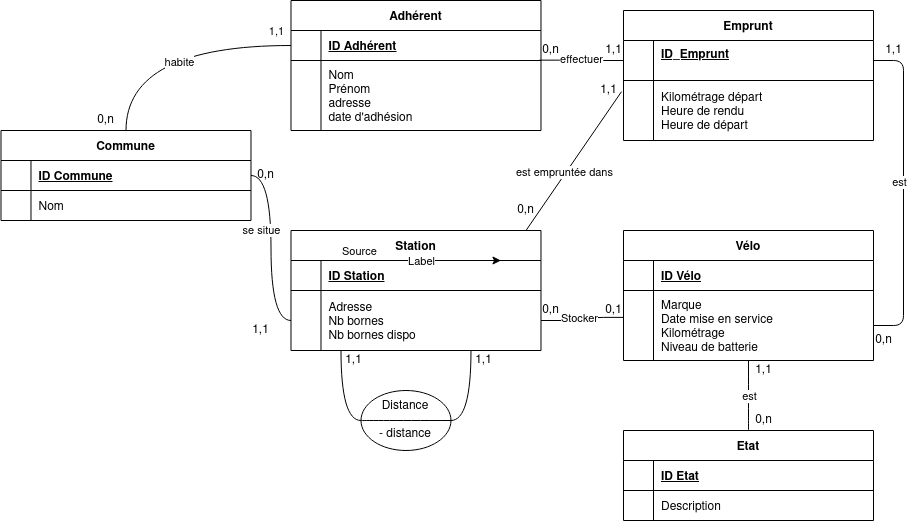
\includegraphics[scale=0.5]{img/entite_association}
    \caption{Schéma entité-association}
    \label{fig:entite}
  \end{figure}

  \subsection{Schéma relationnel}\label{sec:relationel}

  Dans notre modèle entité association, on retrouve premièrement des associations 1, n.
  Dans ce cas la, la traduction au modèle relationnel se fait en définissant comme clé étrangère, pour l'entité de côté 1,
  la clé primaire de l'entité de côté n.
  Le deuxième cas que l'on retrouve est celui de la relation de cardinalité 1, 1 qu'est \textit{Distance} entre deux entité \texttt{STATION}.
  Celle-ci se retrouvera donc comme une table dans le modèle relationnel avec comme clé primaire les 2 clés étrangères des
  deux stations.
  Nous avons donc finalement le modèle relationnel suivant :\\
  \begin{itemize}
    \item ADHERENT (\underline{ID adherent}, nom, prénom, adresse, date d'adhésion, #ID commune (non nul));
    \item COMMUNE (\underline{ID commune}, nom);
    \item STATION (\underline{ID station}, adresse, nb bornes, nb bornes dispo, #ID commune (non nul));
    \item DISTANCE (\underline{#ID station1 (non nul), #ID station2 (non nul)}, distance);
    \item VELO (\underline{ID vélo}, marque, date mise en service, kilométrage, niveau de batterie, #ID station, #ID état (non nul));
    \item ETAT (\underline{ID_état}, description);
    \item EMPRUNT (\underline{ID emprunt}, km départ, heure)
  \end{itemize}
  \begin{figure}[!h]
    \centering
    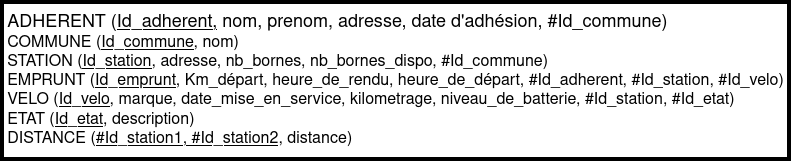
\includegraphics[scale=0.5]{img/schema_relationel}
    \caption{Schéma relationnel de la base}
    \label{fig:relat}
  \end{figure}

  \section{Implémentation}\label{sec:implementation}
  Maintenant que nous disposons de notre schéma relationel en 3\ieme{} forme,
  \subsection{Création et remplissage de la base de donnée}\label{subsec:crea}
  \subsubsection{Les tables}
  \subsubsection{Les Triggers}
  \subsubsection{Les procédures}
  
  \subsection{Implémentation des requêtes}\label{subsec:requete}
  \subsubsection{Les consultations}
  \subsubsection{Les statistiques}
  
  \section{Utilisation}\label{sec:utili}
  
  Une fois nos bases de données implémentées, nous pouvions les manipuler depuis le terminal. Celle-ci étant peu ergonomique, nous avons décidé de développer une interface web.
  
  \subsection{Description de l'interface utilisateur}\label{subsec:desc}
  
  Le projet est basé sur 2 serveurs. Le premier est un serveur MariaDB, il s'occupe de gérer la base. Le deuxième est un serveur NodeJS qui fournit l'interface graphique du projet. \\
 
  Nous avons construit le serveur Node afin qu'il mettre à disposition des API pour la page principale. Pour cela, nous avons utilisé le module express. Ce dernier permet de gérer très facilement le rootage, en utilisant des expressions régulières notamment, et de répondre différemment suivant la méthode de requête utilisée. C'est le serveur NodeJS qui s'occupe d'envoyer les requêtes au serveur MariaDB.
  Pour le rendu, nous avons utilisé Jquery et Bootstrap, afin de manipuler plus efficacement le DOM et de désigner rapidement l'interface. Pour l'affichage des tables, le plug-in Datatables s'est montré particulièrement efficace. \\
  
  La procédure d'installation ainsi que les dépendances du projet sont détaillées dans le fichier \mbox{\textit{/front/README.md}}.
  
  \subsection{Possibilité et utilisations}\label{subsec:possib}
  
La page principale est découpée en 4 sections :
  \begin{itemize}
  \item Une section d'affichage du contenu d'une table, avec des boutons d'édition et de suppression
  \item Une fenêtre d'édition qui souvre après sélection d'une ligne
  \item Une section d'affichage des statistiques du projet
  \item Un formulaire pour insérer des éléments dans la table sélectionnée \\
\end{itemize}

L'ensemble des tables peut être affiché et modifié (sauf la table \textit{distance}), ainsi que leurs champs, excepté leurs clés primaires. Nous avons décidé de ne pas pouvoir modifier la table distance afin de garder la cohérence de celle-ci. Pour l'affichage des statistiques, nous avons implémenté les indicateurs précisés dans le sujet.

Pour l'insertion d'éléments dans la base, nous avons ajouté au formulaire uniquement les champs strictement nécessaires. Le calcul des clés primaires, la création et le rendu d'un emprunt se font via des procédures. Nous avons par exemple uniquement besoin de l'id de l'adhérent et du vélo utilisé pour créer un emprunt, le reste des champs est calculé automatiquement. Notons qu'il n'y a aucune vérification du les informations saisies, le projet est donc vulnérable aux injections SQL.

  \section{Conclusion}\label{sec:ccl}
\end{document}